\chapter{Appendix}
\minitoc
\notesurl{introappendix}


\section{Directories in the Pi's root filesystem}
\label{appendix:pidirs}

\begin{table}
\begin{tabular}{lp{12cm}}
\hline
Directory & Description\\
\hline
boot & Contains the Linux kernel and other low-level packages needed to get the Pi to boot.\\
& \\
bin & Contains the binary executables for basic commands such as \totype{ls} and \totype{pwd}.\\
& \\
dev & This is a virtual directory that represents devices connected to the Pi as though they were files that you can read from and write to. \\
 & \\
etc & Contains configuration files used by various programs, and also the names and encrypted passwords of users\\
 & \\
home & Each user gets their own subdirectory of \fname{home}. \\
 &\\
lib & This is where \textit{libraries} are stored; these are bits of code that are shared between several programs.\\
 & \\
lost+found & If something bad happens and the system crashes half way through doing something, it will put a copy of files that it knows are in a broken state here.\\
media & When you mount removable storage devices such as USB memory stickets, they will appear as filesystems here.\\
 & \\
mnt & This directory is used to mount storage devices. \\
& \\
opt & When you install optional software that's not considered part of the operating system, it usually ends up here.\\
& \\
proc & Like dev, this is a virtual directory. This one contains accounting information about the various processes that are running on your Pi.\\
& \\
selinux & Contains utility files relating to Security Enhance Linux.\\
& \\
sbin & This contains special executable binary files associated with system maintenance.\\
& \\
sys & Various files needed by the operating system.\\
& \\
tmp & Many programs need to create temporary files as part of their execution; they go here, and get deleted when the system reboots.\\
& \\
usr & User-accessible programs and bits of configuration.\\
& \\
var & Another virtual directory, used by programs to store variables.\\
\hline
\end{tabular}
\caption{Standard Linux system directories.}\label{table-dirs}
\end{table}

\section{A Map Of Colossal Cave}
\label{appendix:colossal-map}
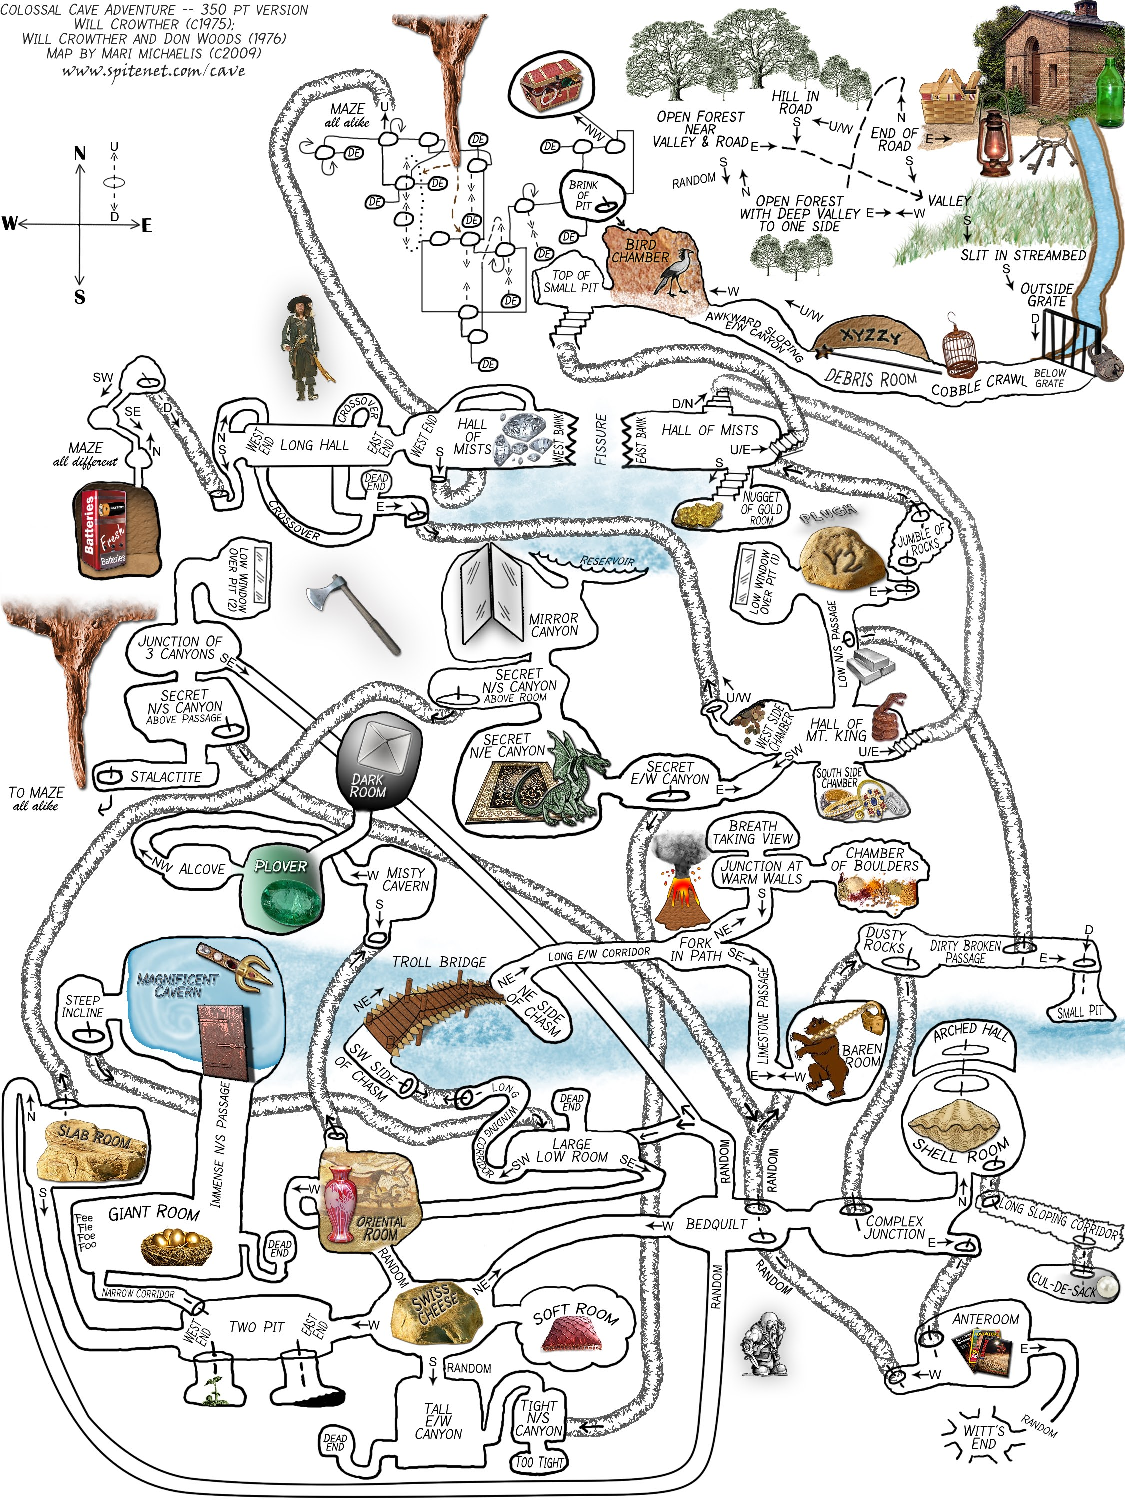
\includegraphics[width=13cm]{images/ColossalCaveAdventureMap}\\
\\
This map of Colossal Cave is reproduced here by kind permission of its author, Mari Michaelis. This is the `spoilers' version of the map, and contains clues as to how to solve the various puzzles in the game. If you want to play the game for real, you probably should make your own map, or at least use the spoiler-free version of the map available at \url{www.spitenet.com/cave}.

\section{Basic HTML}
\label{appendix:simplehtml}

\wikipedia{HTML}{HTML} is a markup language used for creating web pages. It
encodes the structure and content of a page, and it's interpreted by a
web browser in order to display the page. This section gives a very
quick overview of a few basic HTML features, and omits a lot of stuff,
most notably \wikipedia{CSS}{CSS} which is used to style the visual
appearance of the content encoded by HTML. You'll meet CSS properly,
later in the course.

For a complete HTML tutorial, see, for example,
\urlnop{www.w3schools.com/html}.

\subsection{Basic page structure}

Here's the basic structure of a webpage.

\begin{ttoutenv}
<html>
<head>
<body>
Hello world!
</body>
</head>
</html>
\end{ttoutenv}

Each construction in angle-brackets, such as \verb|<body>| is called a
`tag'. Most tags come in in pairs, as in the above example, where
\verb|<body>| and \verb|</body>| delimit the `body' of the page, which
in this case it's simply the text `Hello World!'.

\subsection{Page structure}

Let's expand the body of the page, first to introduce some section
headings, and add some paragraphs:

\begin{ttoutenv}
<body>
<h1>This is a level-1 section heading</h1>

<p>Hello world! (paragraph 1) </p>

<p>This is paragraph 2 </p>
</body>
\end{ttoutenv}

The \verb|<h1>| tag specifies the start of a new section. The browser
will render this as larger-than-usual text, and add some vertical
space around it. The \verb|<p>| tag says `start a new paragraph', and
\verb|</p>| says `end the paragraph', which again the browser renders
with a bit of vertical space. You probably get the idea.

Here's how to make a bulleted list (\verb||<ul>| stands for `unordered
list'; \verb|<li>| means `list item'):

\begin{ttoutenv}
My hobbies are:
<ul>
<li>astronomy</li>
<li>gastronomy</li>
<li>hippogastronomy</li>
</ul>
\end{ttoutenv}

You can make a numbered list with \verb|<ol>...</ol>|.

\subsection{Hyperlinks}

One of the most powerful features of HTML is of course to create hyperlinks to
other pages, using the \verb|<a>| tag, as follows:

\begin{ttoutenv}
<a href="web page address">text for link</a>.
\end{ttoutenv}

For example:

\begin{ttoutenv}
My hobby is writing for <a href="http://en.wikipedia.org/">wikipedia</a>.
\end{ttoutenv}

\section{Using USB sticks in Linux}
\label{appendix:usingUSB}

Using a USB drive with the Pi presents an interesting challenge. If you are running the graphical LXDE environment, then you can just plug a USB Drive into one of the USB ports, and a handy filebrowser window will appear, allowing you to copy files on and off the drive, and then eject it when you're done much as you would do in Windows or OS X. But the problem is that the Pi only has two USB ports, and the chances are that both of these will be in use with the keyboard and mouse. Oh dear. You could of course use a USB hub to get around this, but unless you happen to have one handy you're a bit stuck.

Fortunately, it's quite possible to mount USB devices using the command line, and by dropping back to console mode, you can unplug the mouse to free up a USB slot. Unfortunately, the process of mounting a USB device `manually' is a little fiddly. But follow these instructions and all will be well.

The first thing you'll need to do is to find out what the Pi thinks your USB device is called. To do this, we'll need to use the \ttout{tail} command to look at a system log and spot the name of the device when you plug it in. Type:

\begin{ttoutenv}
tail -f /var/log/messages
\end{ttoutenv}

and then plug in your USB drive. You'll see a series of lines appear, containing text like 'New USB device found', and after these a line which says `sda: sda1' (actually 'sda1' may be a different number on your Pi, but unless you've connected other USB storage devices it will most-likely be sda1). Note this number down, you will need it in a moment.

The \ttout{tail} command behaves a little like \ttout{less} in that it displays the contents of a file (in this case, one of the systems log files); the difference is that tail allows you to see the last few lines of a file instead of starting from the beginning. The \ttout{-f} switch to \ttout{tail} tells it to `follow' a file, that is to continue to watch the file and to display any new lines that get appended to the end of that file (without the switch, \ttout{tail} just displays the lines and then quits).

Now that you have the sda number from the log file, quit \ttout{tail} using \ctrl{c}.

% TODO Finish this description - currently no information on how to mount
% TODO USB devices on the command line. PW
